\section{Laboratory work implementation}

\subsection{Tasks and Points}

\begin{description}
	\item[Task-ul] nr. 1
\\Sa se realizeze un program ce va incrementa/decrementa un numar.
\\Se vor utiliza următoarele obiecte (în afara formei):
\begin{itemize}
\item	două butoane (Button 1 şi 2) pentru incrementarea (UP) respectiv decrementarea (DOWN) a unei variabile întregi i ;
\item	un buton (Button 3) pentru ieţirea din program (Exit);
\item	o casetă de editare (Edit1) unde se va afişa  valoarea variabilei i;
\item	două etichete (Label1 şi 2) pentru afişarea textului „Incrementare decrementare contor.” Respectiv a sensului de variaţie a variabilei i din caseta Edit1;
\item	în caption-ul formei se va afişa textul „ MIDPS 1- A”;
\item	fiecare obiect va avea hint-ul activ completat corespunzător .
\end{description}

	\item[Task-ul] nr. 2
\\  Se  elaborează  un program pentru realizarea unui cronometru.
\\Se vor utiliza următoarele obiecte:
\begin{itemize}
\item    o formă (Form1) pe care sunt dispuse celelalte obiecte şi în Caption-ul căreia se va afişa textul „MIDPS”;
\item	patru butoane (Button 1, 2, 3 , 4) cu următoarele funcţii: 
\item	Button1 – pornirea cronometrului( Caption Start);
\item	Button2 – oprirea cronometrului( Caption Stop);
\item	Button3 – iniţializarea cronometrului( Caption Zero);
\item	Button4 – ieşirea din program (Caption Exit).
\item	două timere (Timer1 şi Timer2)  cu următoarele funcţii
\item	Timer1 (Interval=1000 ms) utilizat la afişarea timpului curent;
\item	Timer2 (Interval=100 ms) utilizat pentru cronometru;
\item	două casete de editare (Edit1 si Edit2) utilizate pentru :
\item	Edit1 - afisarea datei si orei curente;
\item	Edit2 - afişarea timpului cronometrat;
\item	două etichete (Label1 si Label2) cu Caption-ul conform figurii 2.4
Observaţii: 
	\item	din primele trei butoane, la un un moment dat va fi  activ unul singur;
\item	fiecare obiect va avea hint-ul activ completat corespunzător;
\end{itemize}
	\item[Task-ul] nr. 3 
\\Se  elaborează  un program pentru realizarea a două elemente de afişare (bargraf şi diagramă cu avans continuu) pe care sunt dispuse următoarele obiecte:
\begin{itemize}
\item o formă (Form1)  în Caption-ul căreia se va afişa textul „MIDPS;
\item	trei butoane (Button 1, 2, 3 ) cu următoarele funcţii: 
\item	Buton1 – activarea afişării în diagramă şi în bargraf ( Caption Start);
\item	Buton2 – oprirea afişării în diagramă şi în bargraf ( Caption Stop);
\item	Buton3 – ieşirea din program (Caption Exit).
\item	două timere (Timer1 şi Timer2)  cu următoarele funcţii
\item	Timer1 (Interval=1000 ms) utilizat la afişarea timpului curent;
\item	Timer2 (Interval=500 ms) pentru intervalul de afişare în diagramă şi în bargraf;
\item	o casetă de editare (Edit1) utilizată pentru afişarea datei si orei curente;
\item	două etichete (Label1 si Label2) cu Caption-ul conform figurii 4.4
	
	Observaţii: 
	\item	din primele două butoane, la un un moment dat va fi  activ unul singur;
\item	fiecare obiect va avea hint-ul activ completat corespunzător;
\item	valoarea numerică ce se va afişa în cele două elemente grafice se obţine cu funcţia random după care numărul generat se va converti în pixeli ţinându-se cont de înălţimea comună a graficului şi bargrafului
\item	pentru realizarea bargrafului se vor utiliza două obiecte de tip TPanel de culori diferite care se vor suparpune;
\item	pentru desenarea graficului se vor utiliza funcţiile MoveTo, LineTo iar pentru avansul acestuia funcţia CopyRect.

\end{itemize}
\end{description}

\subsection{Analiza lucrarii de laborator}

Link la repozitoriu: https://github.com/Erdboden/MIDPS_141$
\\Task-ul  1:
\\Din bara de meniiu standard am selectat 3 butoane, un editbox si doua labels.
Apasind dublu click pe pe primul buton care va fi incrementare(up) s-a deschis editorul in care automat a aparut si event-ul butonului. Prin apelarea numelui 
editboxului.Text, il putem edita. Astfel cream o variabila integer "i", si o plasam in editbox: Edit1.Text = ++i;
\\Acelasi lucru procedam si cu al doilea buton(down) pentru decrementare.
Pentru butonul 3, in event-ul lui scriem codul exit(42) pentru iesire din program.
\\Deasemenea in butonul 1 si 2  inscriem Label2.Caption=("Increment i"); si respectiv Label2.Caption=("Decrement i"); pentru schimbarea textului in label2.
Am descris hinturile si am dat denumire ferestrei.

\\Task-ul 2:
\\Am selectat 4 butoane, 2 timere din meniul System, 2 editbox-uri si 2 labels. In inspector al obiectului Timer, pentru primul am setat intervalul 1000, iar pentru al 2-lea 100. Pentru primul editbox, atasam primul timer cu intervalul 1000 pentru a vizualiza data si ora curenta. Editbox-ul nr 2 va fi legat de al doilea timer cu intervalul 100, pentru vizualizarea unui cronometru. Milisecundele doar se vor incrementa, cind numarul ms. vor atinge cifra 10, urmeaza incrementarea secundelor. Minutele se incrementeaza la 60 secunde. la indeplinirea acestor conditii secundele sau milisecundele se vor intoarce la 0.

\\Task-ul 3:
\\Am selectat 3 butoane, de pornirea timerului, oprirea lui si iesire din program. Timerul are intervalul 500 si este legat de bargraf(panela din fata) si paintbox.
Timerul nr. 1 este atasat de primul editbox unde se va afisa data si ora curenta. Prin apasarea tastei Start, timer1 se porneste. in intervalul 500 ms se va genera un numar random care se va atribui inaltimei bargrafului. la intervalul de 500 bargraful va oscila pe verticala. Aceeasi variabila este transmisa canvasului din paintbox in care se va trasa o linie prin functia LineTo(x+1,y) unde x este punctul final pe orizontala si y(random) punctul final pe verticala.
Dupa trasarea liniei se copie zona dreptunghiului unde a fost trasata linia si se muta la stinga. Linia urmatoare va incepe trasarea din punctul final al liniei precedente.
Grid-ul din paintbox a fost creat cu ajutorul functiei FloodFill indicind si stilul de hasurare bsCross.

 
\subsection{Imagini}

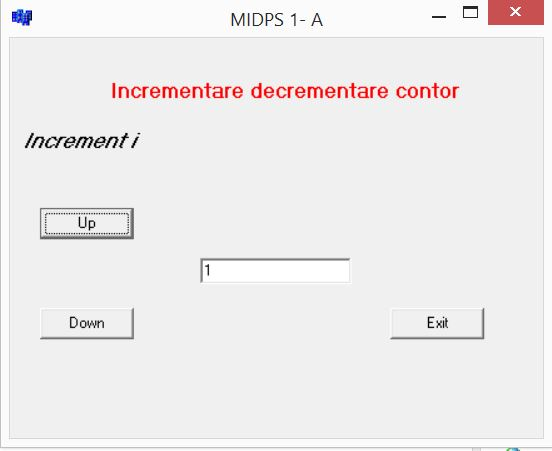
\includegraphics{1.jpg}
\\
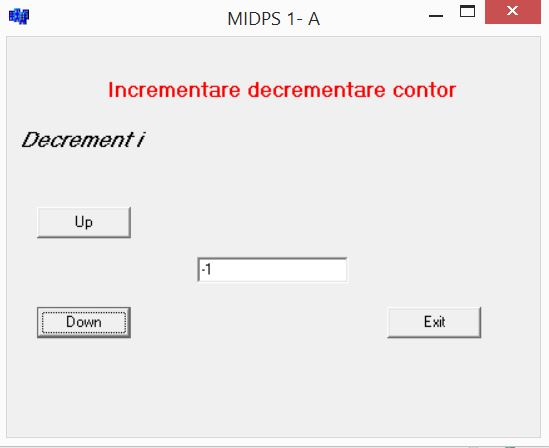
\includegraphics{2.jpg}
\\
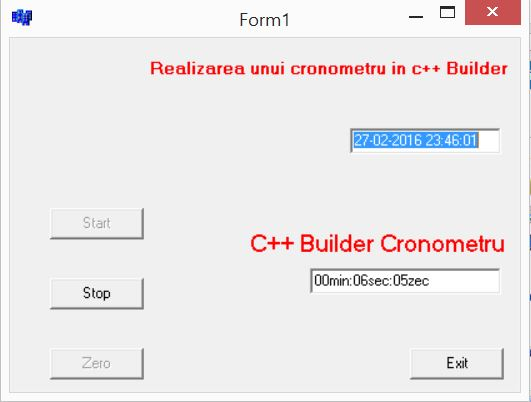
\includegraphics{3.jpg}
\\
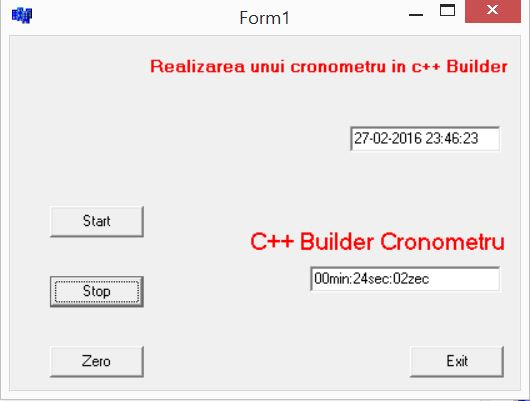
\includegraphics{4.jpg}
\\
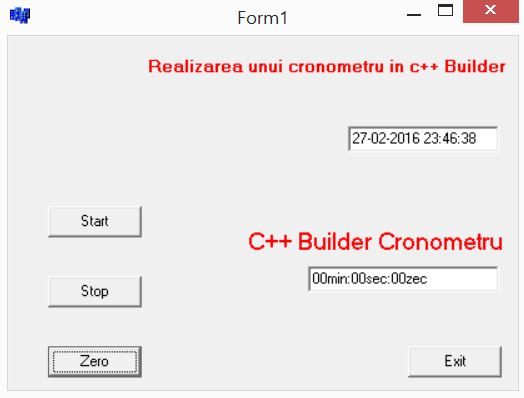
\includegraphics{5.jpg}
\\
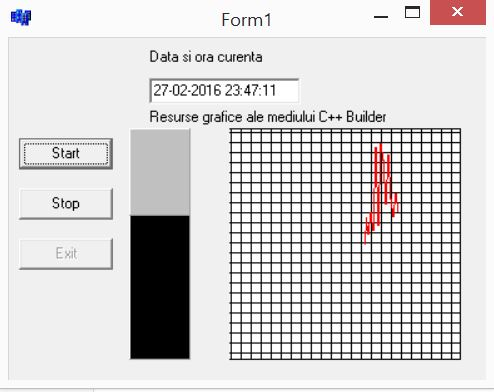
\includegraphics{6.jpg}
\\
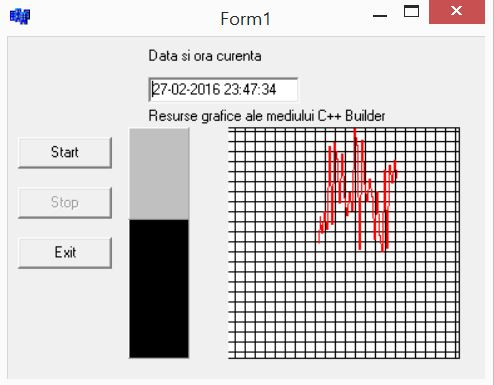
\includegraphics{7.jpg}
\clearpage